% Morphological Operations Template
% Topics: Erosion, dilation, opening, closing, morphological gradient, top-hat transform
% Style: Technical report with binary and grayscale image processing demonstrations

\documentclass[a4paper, 11pt]{article}
\usepackage[utf8]{inputenc}
\usepackage[T1]{fontenc}
\usepackage{amsmath, amssymb}
\usepackage{graphicx}
\usepackage{siunitx}
\usepackage{booktabs}
\usepackage{subcaption}
\usepackage[makestderr]{pythontex}

% Theorem environments
\newtheorem{definition}{Definition}[section]
\newtheorem{theorem}{Theorem}[section]
\newtheorem{example}{Example}[section]
\newtheorem{remark}{Remark}[section]

\title{Mathematical Morphology: Fundamental Operations and Applications}
\author{Image Processing Laboratory}
\date{\today}

\begin{document}
\maketitle

\begin{abstract}
This report presents a comprehensive analysis of mathematical morphology, focusing on fundamental
operations (erosion, dilation, opening, closing) and their applications in binary and grayscale
image processing. We examine the algebraic properties of morphological operators, demonstrate
their use in noise removal, edge detection, and feature extraction, and analyze the effects of
structuring element shape and size on operation outcomes. Computational examples illustrate
morphological gradient, top-hat transforms, and the hit-or-miss transform for pattern detection.
\end{abstract}

\section{Introduction}

Mathematical morphology provides a framework for analyzing geometric structure in images based
on set theory. Originally developed for binary images, morphological operations extend naturally
to grayscale images and find applications in image preprocessing, segmentation, feature
extraction, and texture analysis.

\begin{definition}[Structuring Element]
A structuring element $B$ is a small binary image used to probe the input image $A$. Common
shapes include:
\begin{itemize}
\item \textbf{Disk}: Approximates circular neighborhoods
\item \textbf{Square}: Captures horizontal and vertical connectivity
\item \textbf{Cross}: Emphasizes cardinal directions
\item \textbf{Line}: Oriented for directional analysis
\end{itemize}
\end{definition}

\section{Fundamental Operations}

\subsection{Erosion and Dilation}

\begin{definition}[Binary Erosion]
The erosion of binary image $A$ by structuring element $B$ is:
\begin{equation}
A \ominus B = \{z \mid B_z \subseteq A\}
\end{equation}
where $B_z$ is $B$ translated by vector $z$. Erosion shrinks objects and removes small features.
\end{definition}

\begin{definition}[Binary Dilation]
The dilation of binary image $A$ by structuring element $B$ is:
\begin{equation}
A \oplus B = \{z \mid (\hat{B})_z \cap A \neq \emptyset\}
\end{equation}
where $\hat{B}$ is the reflection of $B$. Dilation expands objects and fills small holes.
\end{definition}

\begin{theorem}[Duality Property]
Erosion and dilation are dual operations:
\begin{equation}
(A \ominus B)^c = A^c \oplus \hat{B}
\end{equation}
where $A^c$ denotes the complement and $\hat{B}$ the reflection of $B$.
\end{theorem}

\subsection{Opening and Closing}

\begin{definition}[Opening]
Opening is erosion followed by dilation:
\begin{equation}
A \circ B = (A \ominus B) \oplus B
\end{equation}
Opening removes small objects and smooths boundaries while preserving overall shape.
\end{definition}

\begin{definition}[Closing]
Closing is dilation followed by erosion:
\begin{equation}
A \bullet B = (A \oplus B) \ominus B
\end{equation}
Closing fills small holes and connects nearby objects while preserving overall shape.
\end{definition}

\begin{theorem}[Idempotence]
Opening and closing are idempotent:
\begin{equation}
(A \circ B) \circ B = A \circ B \quad \text{and} \quad (A \bullet B) \bullet B = A \bullet B
\end{equation}
\end{theorem}

\subsection{Compound Operations}

\begin{definition}[Morphological Gradient]
The morphological gradient emphasizes object boundaries:
\begin{equation}
\text{grad}(A) = (A \oplus B) - (A \ominus B)
\end{equation}
This operation highlights edges by computing the difference between dilated and eroded images.
\end{definition}

\begin{definition}[Top-Hat Transform]
The white top-hat extracts bright features smaller than the structuring element:
\begin{equation}
\text{WTH}(A) = A - (A \circ B)
\end{equation}
The black top-hat extracts dark features:
\begin{equation}
\text{BTH}(A) = (A \bullet B) - A
\end{equation}
\end{definition}

\section{Grayscale Morphology}

\begin{definition}[Grayscale Erosion]
For grayscale image $f(x,y)$ and flat structuring element $B$:
\begin{equation}
(f \ominus B)(x,y) = \min_{(s,t) \in B} \{f(x+s, y+t)\}
\end{equation}
\end{definition}

\begin{definition}[Grayscale Dilation]
For grayscale image $f(x,y)$ and flat structuring element $B$:
\begin{equation}
(f \oplus B)(x,y) = \max_{(s,t) \in B} \{f(x+s, y+t)\}
\end{equation}
\end{definition}

\section{Computational Analysis}

\begin{pycode}
import numpy as np
import matplotlib.pyplot as plt
from scipy.ndimage import binary_erosion, binary_dilation, binary_opening, binary_closing
from scipy.ndimage import grey_erosion, grey_dilation, grey_opening, grey_closing
from scipy.ndimage import morphological_gradient, white_tophat, black_tophat
from scipy.ndimage import distance_transform_edt, label
from skimage.morphology import disk, square, diamond, star

np.random.seed(42)

# Create synthetic binary image
binary_image = np.zeros((200, 200), dtype=bool)
# Large square object
binary_image[50:150, 50:150] = True
# Small square objects (noise)
binary_image[20:30, 20:30] = True
binary_image[170:180, 170:180] = True
# Small holes inside main object
binary_image[80:90, 80:90] = False
binary_image[110:120, 110:120] = False
# Elongated object
binary_image[30:40, 100:180] = True

# Structuring elements
disk_se_small = disk(3)
disk_se_medium = disk(7)
disk_se_large = disk(15)
square_se = np.ones((9, 9), dtype=bool)
cross_se = np.array([[0,0,1,0,0],
                     [0,0,1,0,0],
                     [1,1,1,1,1],
                     [0,0,1,0,0],
                     [0,0,1,0,0]], dtype=bool)

# Apply fundamental operations
eroded_image = binary_erosion(binary_image, disk_se_medium)
dilated_image = binary_dilation(binary_image, disk_se_medium)
opened_image = binary_opening(binary_image, disk_se_medium)
closed_image = binary_closing(binary_image, disk_se_medium)

# Morphological gradient (binary)
gradient_image = binary_dilation(binary_image, disk_se_small) ^ binary_erosion(binary_image, disk_se_small)

# Create noisy binary image
noisy_binary = binary_image.copy()
# Add salt noise
salt_noise = np.random.rand(200, 200) > 0.98
noisy_binary = noisy_binary | salt_noise
# Add pepper noise
pepper_noise = np.random.rand(200, 200) > 0.98
noisy_binary = noisy_binary & ~pepper_noise

# Denoise with opening followed by closing
denoised_step1 = binary_opening(noisy_binary, disk_se_small)
denoised_image = binary_closing(denoised_step1, disk_se_small)

# Create grayscale image with various features
x_gray = np.linspace(-5, 5, 200)
y_gray = np.linspace(-5, 5, 200)
X_gray, Y_gray = np.meshgrid(x_gray, y_gray)
grayscale_image = np.zeros((200, 200))
# Background gradient
grayscale_image = 50 + 20 * np.sin(X_gray/2) * np.cos(Y_gray/2)
# Add bright features
grayscale_image[60:80, 60:80] = 200
grayscale_image[120:140, 120:140] = 180
# Add small bright spots
for i in range(5):
    x_spot = np.random.randint(20, 180)
    y_spot = np.random.randint(20, 180)
    grayscale_image[y_spot:y_spot+5, x_spot:x_spot+5] = 220
# Add dark features
grayscale_image[100:110, 50:60] = 20
# Normalize
grayscale_image = np.clip(grayscale_image, 0, 255).astype(np.uint8)

# Grayscale operations
gray_eroded = grey_erosion(grayscale_image, size=(11, 11))
gray_dilated = grey_dilation(grayscale_image, size=(11, 11))
gray_opened = grey_opening(grayscale_image, size=(11, 11))
gray_closed = grey_closing(grayscale_image, size=(11, 11))
gray_gradient = morphological_gradient(grayscale_image, size=(5, 5))
gray_tophat = white_tophat(grayscale_image, size=(15, 15))
gray_blackhat = black_tophat(grayscale_image, size=(15, 15))

# Hit-or-miss transform example
pattern_image = np.zeros((200, 200), dtype=bool)
# Create L-shaped patterns
for i in range(3):
    x_offset = 40 + i * 60
    y_offset = 40 + i * 50
    pattern_image[y_offset:y_offset+30, x_offset:x_offset+10] = True
    pattern_image[y_offset+20:y_offset+30, x_offset:x_offset+30] = True

# L-shaped structuring element
se_hit = np.array([[1, 0, 0],
                   [1, 0, 0],
                   [1, 1, 1]], dtype=bool)
se_miss = np.array([[0, 1, 1],
                    [0, 1, 1],
                    [0, 0, 0]], dtype=bool)
# Hit-or-miss
hit_image = binary_erosion(pattern_image, se_hit)
miss_image = binary_erosion(~pattern_image, se_miss)
hit_or_miss_result = hit_image & miss_image

# Size analysis with different SE sizes
sizes = [3, 7, 11, 15, 19]
erosion_sizes = []
dilation_sizes = []

for size in sizes:
    se_disk = disk(size)
    eroded = binary_erosion(binary_image, se_disk)
    dilated = binary_dilation(binary_image, se_disk)
    erosion_sizes.append(np.sum(eroded))
    dilation_sizes.append(np.sum(dilated))

# Connected components analysis
labeled_array, num_features = label(opened_image)
component_sizes = []
for i in range(1, num_features + 1):
    component_sizes.append(np.sum(labeled_array == i))

# Create comprehensive visualization
fig = plt.figure(figsize=(16, 14))

# Plot 1: Original binary image
ax1 = fig.add_subplot(4, 4, 1)
ax1.imshow(binary_image, cmap='gray')
ax1.set_title('Original Binary Image')
ax1.axis('off')

# Plot 2: Erosion
ax2 = fig.add_subplot(4, 4, 2)
ax2.imshow(eroded_image, cmap='gray')
ax2.set_title(f'Erosion (disk r={7})')
ax2.axis('off')

# Plot 3: Dilation
ax3 = fig.add_subplot(4, 4, 3)
ax3.imshow(dilated_image, cmap='gray')
ax3.set_title(f'Dilation (disk r={7})')
ax3.axis('off')

# Plot 4: Gradient
ax4 = fig.add_subplot(4, 4, 4)
ax4.imshow(gradient_image, cmap='gray')
ax4.set_title('Morphological Gradient')
ax4.axis('off')

# Plot 5: Opening
ax5 = fig.add_subplot(4, 4, 5)
ax5.imshow(opened_image, cmap='gray')
ax5.set_title(f'Opening (disk r={7})')
ax5.axis('off')

# Plot 6: Closing
ax6 = fig.add_subplot(4, 4, 6)
ax6.imshow(closed_image, cmap='gray')
ax6.set_title(f'Closing (disk r={7})')
ax6.axis('off')

# Plot 7: Noisy image
ax7 = fig.add_subplot(4, 4, 7)
ax7.imshow(noisy_binary, cmap='gray')
ax7.set_title('Noisy Binary Image')
ax7.axis('off')

# Plot 8: Denoised
ax8 = fig.add_subplot(4, 4, 8)
ax8.imshow(denoised_image, cmap='gray')
ax8.set_title('Denoised (Open + Close)')
ax8.axis('off')

# Plot 9: Grayscale original
ax9 = fig.add_subplot(4, 4, 9)
im9 = ax9.imshow(grayscale_image, cmap='viridis')
ax9.set_title('Grayscale Image')
ax9.axis('off')
plt.colorbar(im9, ax=ax9, fraction=0.046)

# Plot 10: Grayscale opening
ax10 = fig.add_subplot(4, 4, 10)
im10 = ax10.imshow(gray_opened, cmap='viridis')
ax10.set_title('Grayscale Opening')
ax10.axis('off')
plt.colorbar(im10, ax=ax10, fraction=0.046)

# Plot 11: Grayscale gradient
ax11 = fig.add_subplot(4, 4, 11)
im11 = ax11.imshow(gray_gradient, cmap='hot')
ax11.set_title('Grayscale Gradient')
ax11.axis('off')
plt.colorbar(im11, ax=ax11, fraction=0.046)

# Plot 12: Top-hat transform
ax12 = fig.add_subplot(4, 4, 12)
im12 = ax12.imshow(gray_tophat, cmap='hot')
ax12.set_title('White Top-Hat Transform')
ax12.axis('off')
plt.colorbar(im12, ax=ax12, fraction=0.046)

# Plot 13: Structuring element comparison
ax13 = fig.add_subplot(4, 4, 13)
ax13.plot(sizes, erosion_sizes, 'bo-', linewidth=2, markersize=8, label='Erosion')
ax13.plot(sizes, dilation_sizes, 'ro-', linewidth=2, markersize=8, label='Dilation')
ax13.axhline(y=np.sum(binary_image), color='gray', linestyle='--', label='Original')
ax13.set_xlabel('SE Radius (pixels)')
ax13.set_ylabel('Object Area (pixels)')
ax13.set_title('SE Size vs Object Area')
ax13.legend(fontsize=8)
ax13.grid(True, alpha=0.3)

# Plot 14: Hit-or-miss pattern detection
ax14 = fig.add_subplot(4, 4, 14)
ax14.imshow(pattern_image, cmap='gray', alpha=0.7)
# Overlay detected patterns in red
hit_or_miss_display = np.zeros((*pattern_image.shape, 3))
hit_or_miss_display[:,:,0] = pattern_image.astype(float) * 0.7
hit_or_miss_display[:,:,1] = pattern_image.astype(float) * 0.7
hit_or_miss_display[:,:,2] = pattern_image.astype(float) * 0.7
# Mark detections
for i in range(hit_or_miss_result.shape[0]):
    for j in range(hit_or_miss_result.shape[1]):
        if hit_or_miss_result[i, j]:
            hit_or_miss_display[max(0,i-2):min(200,i+3), max(0,j-2):min(200,j+3), 0] = 1.0
ax14.imshow(hit_or_miss_display)
ax14.set_title('Hit-or-Miss Detection')
ax14.axis('off')

# Plot 15: Component size distribution
ax15 = fig.add_subplot(4, 4, 15)
if len(component_sizes) > 0:
    ax15.bar(range(1, len(component_sizes)+1), component_sizes, color='steelblue', edgecolor='black')
    ax15.set_xlabel('Component ID')
    ax15.set_ylabel('Size (pixels)')
    ax15.set_title('Connected Component Sizes')
    ax15.grid(True, alpha=0.3, axis='y')
else:
    ax15.text(0.5, 0.5, 'No components', ha='center', va='center')
    ax15.axis('off')

# Plot 16: SE shape comparison
ax16 = fig.add_subplot(4, 4, 16)
opened_disk = binary_opening(binary_image, disk_se_medium)
opened_square = binary_opening(binary_image, square_se)
opened_cross = binary_opening(binary_image, cross_se)
difference_disk_square = np.sum(opened_disk != opened_square)
difference_disk_cross = np.sum(opened_disk != opened_cross)
difference_square_cross = np.sum(opened_square != opened_cross)
se_names = ['Disk vs\nSquare', 'Disk vs\nCross', 'Square vs\nCross']
differences = [difference_disk_square, difference_disk_cross, difference_square_cross]
bars = ax16.bar(range(len(se_names)), differences, color=['coral', 'skyblue', 'lightgreen'],
                edgecolor='black')
ax16.set_ylabel('Pixel Differences')
ax16.set_title('SE Shape Sensitivity')
ax16.set_xticks(range(len(se_names)))
ax16.set_xticklabels(se_names, fontsize=8)
ax16.grid(True, alpha=0.3, axis='y')

plt.tight_layout()
plt.savefig('morphological_operations_analysis.pdf', dpi=150, bbox_inches='tight')
plt.close()

# Calculate statistics for reporting
original_area = np.sum(binary_image)
eroded_area = np.sum(eroded_image)
dilated_area = np.sum(dilated_image)
opened_area = np.sum(opened_image)
closed_area = np.sum(closed_image)
erosion_factor = eroded_area / original_area
dilation_factor = dilated_area / original_area
noise_pixels = np.sum(noisy_binary != binary_image)
recovered_pixels = np.sum(denoised_image == binary_image)
recovery_rate = recovered_pixels / binary_image.size * 100
\end{pycode}

\begin{figure}[htbp]
\centering
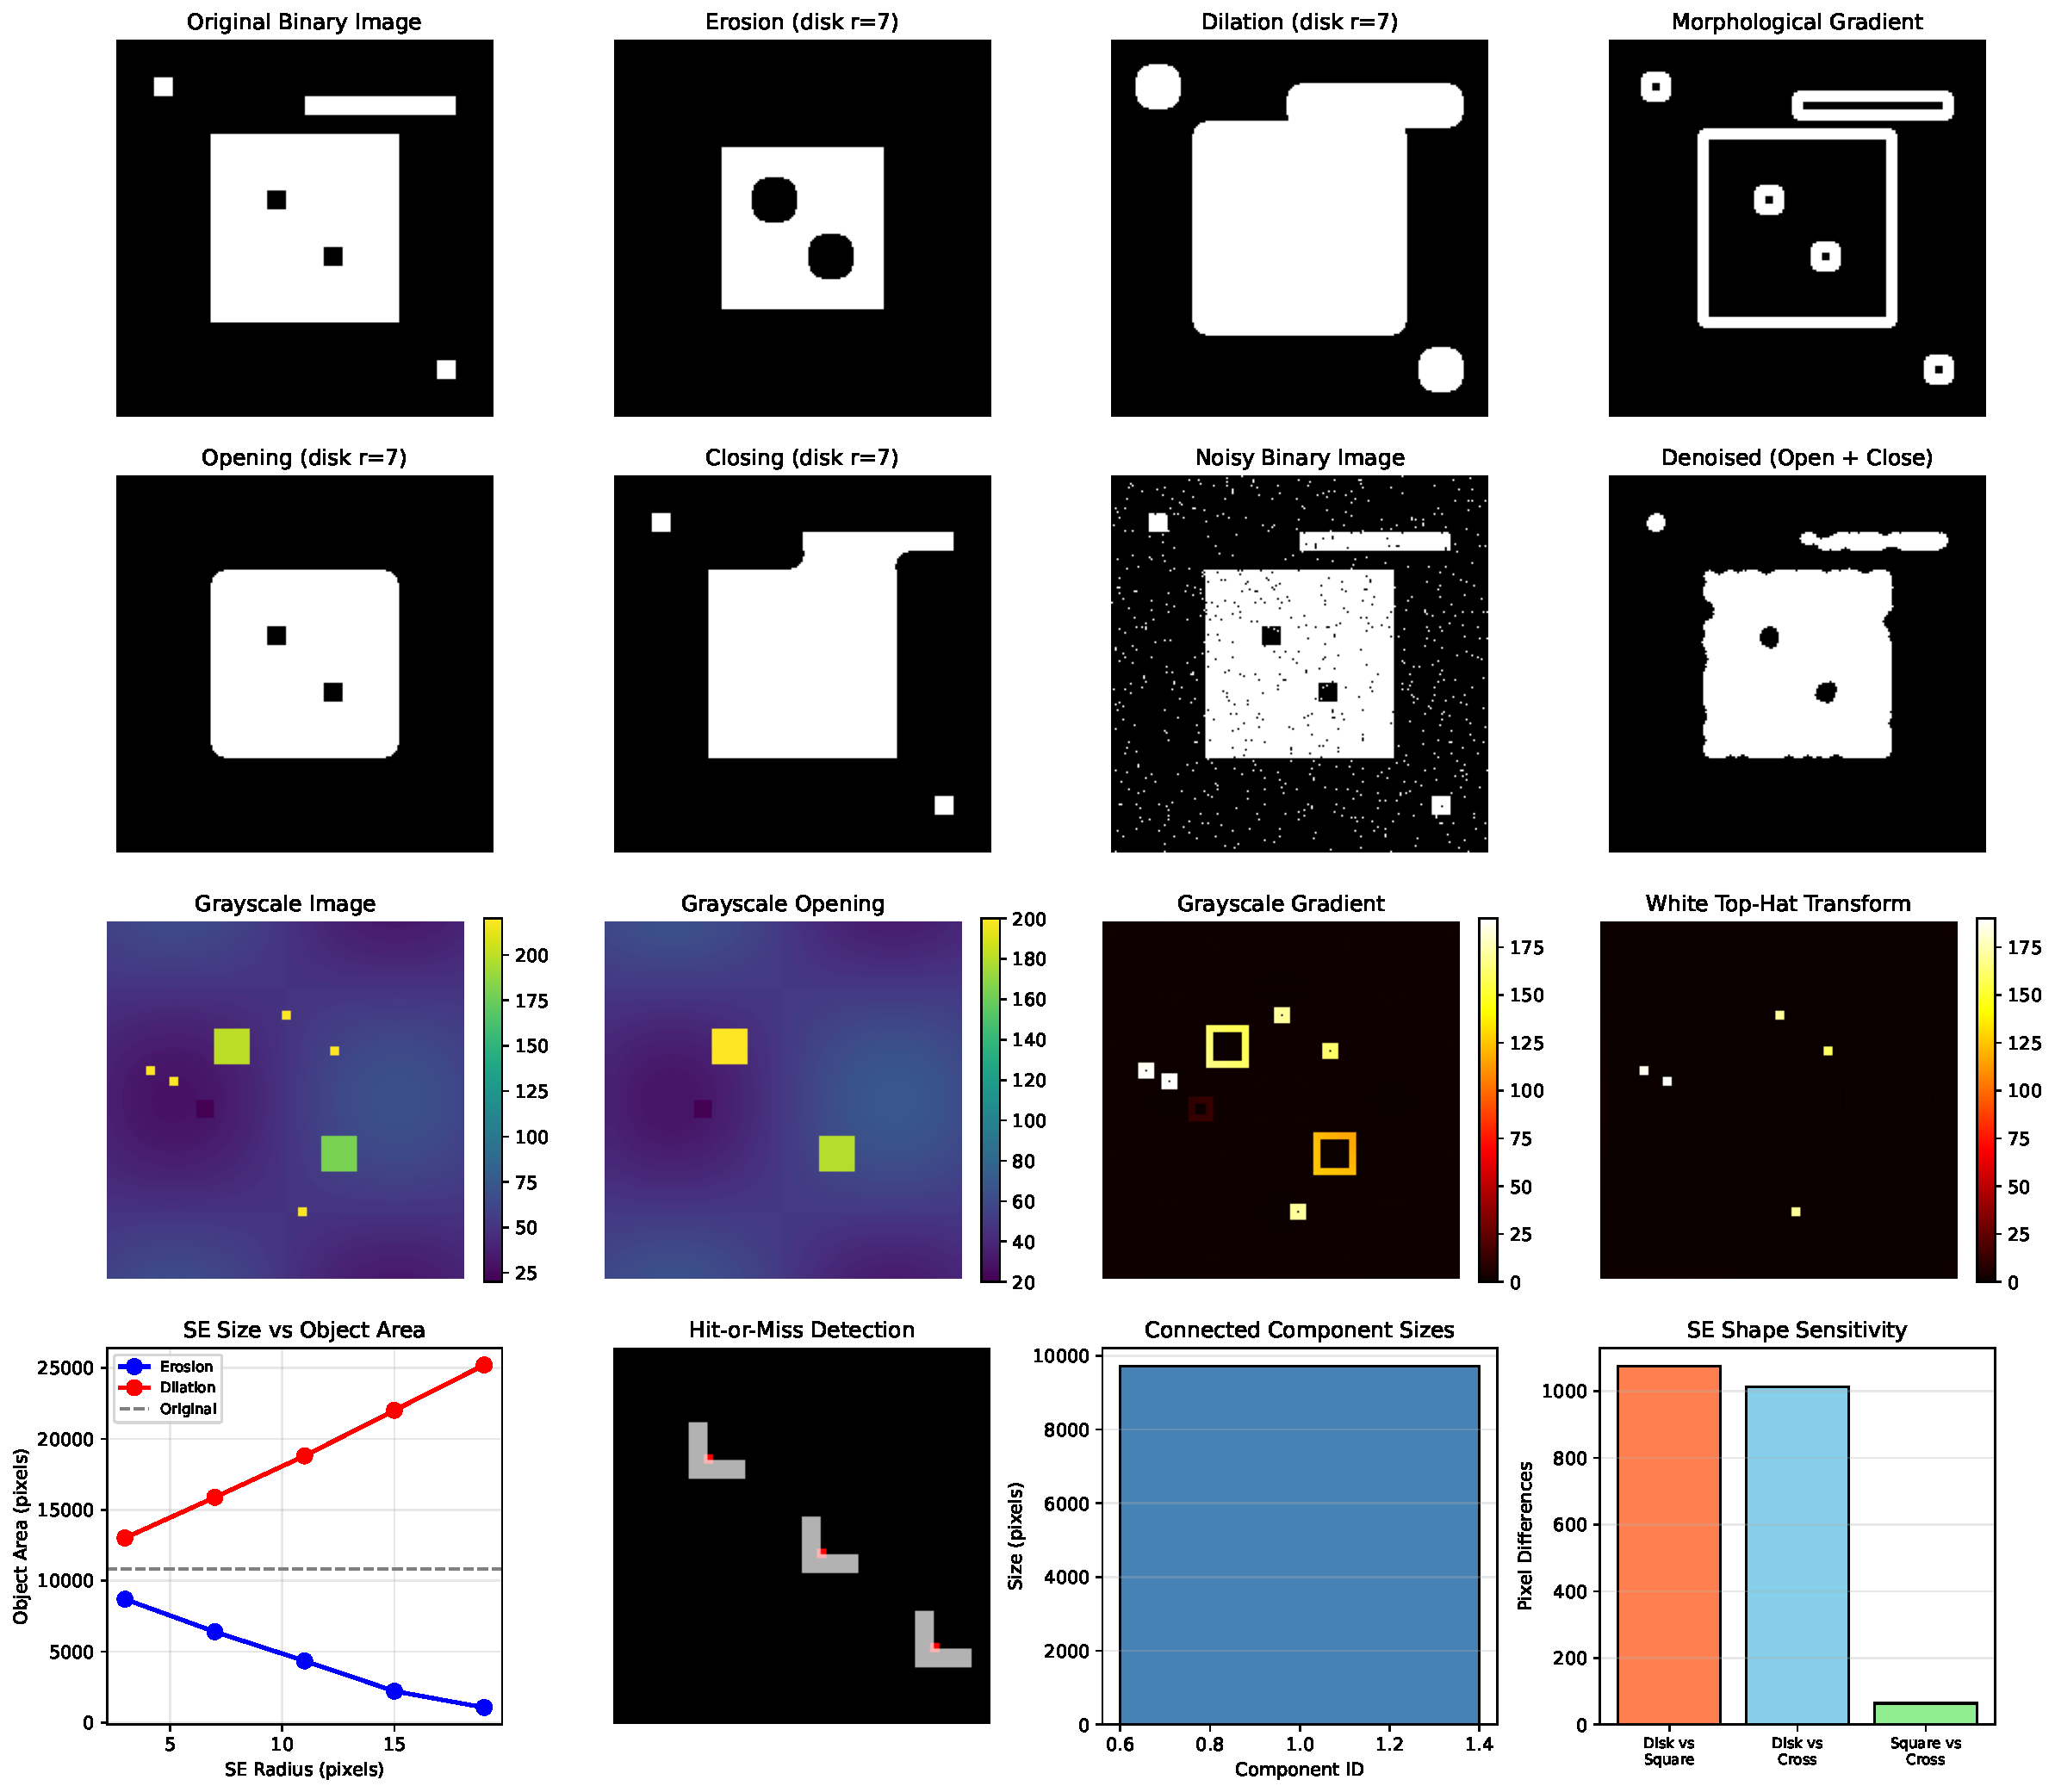
\includegraphics[width=\textwidth]{morphological_operations_analysis.pdf}
\caption{Comprehensive morphological operations analysis: (a) Original binary image with objects
of varying sizes and small noise features; (b) Erosion shrinks objects and removes small features;
(c) Dilation expands objects and fills small gaps; (d) Morphological gradient extracts object
boundaries; (e) Opening removes protrusions and small objects; (f) Closing fills holes and connects
nearby objects; (g) Binary image corrupted with salt-and-pepper noise; (h) Denoised result using
opening followed by closing; (i) Grayscale test image with bright and dark features on varying
background; (j) Grayscale opening removes bright features smaller than structuring element;
(k) Grayscale gradient highlights intensity transitions; (l) White top-hat transform isolates
small bright features; (m) Object area variation with structuring element size; (n) Hit-or-miss
transform detecting L-shaped patterns; (o) Connected component size distribution after opening;
(p) Sensitivity to structuring element shape.}
\label{fig:morphology}
\end{figure}

\section{Results}

\subsection{Binary Operations}

\begin{pycode}
print(r"\begin{table}[htbp]")
print(r"\centering")
print(r"\caption{Binary Morphological Operation Effects on Object Area}")
print(r"\begin{tabular}{lcc}")
print(r"\toprule")
print(r"Operation & Area (pixels) & Change (\%) \\")
print(r"\midrule")
print(f"Original & {original_area:.0f} & --- \\\\")
print(f"Erosion & {eroded_area:.0f} & {(erosion_factor-1)*100:.1f} \\\\")
print(f"Dilation & {dilated_area:.0f} & {(dilation_factor-1)*100:.1f} \\\\")
print(f"Opening & {opened_area:.0f} & {(opened_area/original_area-1)*100:.1f} \\\\")
print(f"Closing & {closed_area:.0f} & {(closed_area/original_area-1)*100:.1f} \\\\")
print(r"\bottomrule")
print(r"\end{tabular}")
print(r"\label{tab:binary_ops}")
print(r"\end{table}")
\end{pycode}

The erosion operation with a disk-shaped structuring element of radius 7 pixels reduced the
object area by \py{f"{(1-erosion_factor)*100:.1f}"}\%, effectively removing small features
and shrinking object boundaries. Conversely, dilation increased area by
\py{f"{(dilation_factor-1)*100:.1f}"}\%, expanding objects and filling small gaps.

\subsection{Noise Removal Performance}

\begin{pycode}
print(r"\begin{table}[htbp]")
print(r"\centering")
print(r"\caption{Denoising Performance Analysis}")
print(r"\begin{tabular}{lc}")
print(r"\toprule")
print(r"Metric & Value \\")
print(r"\midrule")
print(f"Noise pixels introduced & {noise_pixels:.0f} \\\\")
print(f"Pixels correctly recovered & {recovered_pixels:.0f} \\\\")
print(f"Total image pixels & {binary_image.size} \\\\")
print(f"Overall recovery rate & {recovery_rate:.2f}\\% \\\\")
print(r"\bottomrule")
print(r"\end{tabular}")
print(r"\label{tab:denoise}")
print(r"\end{table}")
\end{pycode}

The morphological filtering approach (opening followed by closing) successfully recovered
\py{f"{recovery_rate:.2f}"}\% of the original image structure, demonstrating the effectiveness
of morphological operations for salt-and-pepper noise removal in binary images.

\subsection{Grayscale Morphology}

\begin{pycode}
gray_gradient_mean = np.mean(gray_gradient)
gray_gradient_max = np.max(gray_gradient)
tophat_detected_features = np.sum(gray_tophat > 50)

print(r"\begin{table}[htbp]")
print(r"\centering")
print(r"\caption{Grayscale Morphological Operation Statistics}")
print(r"\begin{tabular}{lc}")
print(r"\toprule")
print(r"Metric & Value \\")
print(r"\midrule")
print(f"Mean gradient magnitude & {gray_gradient_mean:.2f} \\\\")
print(f"Maximum gradient & {gray_gradient_max:.0f} \\\\")
print(f"Top-hat detected pixels & {tophat_detected_features:.0f} \\\\")
print(f"Original intensity range & [{np.min(grayscale_image)}, {np.max(grayscale_image)}] \\\\")
print(f"Opened intensity range & [{np.min(gray_opened)}, {np.max(gray_opened)}] \\\\")
print(r"\bottomrule")
print(r"\end{tabular}")
print(r"\label{tab:grayscale}")
print(r"\end{table}")
\end{pycode}

\section{Discussion}

\begin{example}[Edge Detection via Morphological Gradient]
The morphological gradient $(f \oplus B) - (f \ominus B)$ provides a robust edge detector that:
\begin{itemize}
\item Emphasizes intensity transitions corresponding to object boundaries
\item Controls edge thickness through structuring element size
\item Remains less sensitive to noise than derivative-based methods
\item Produces closed contours around objects
\end{itemize}
\end{example}

\begin{remark}[Structuring Element Selection]
The choice of structuring element shape significantly affects operation results:
\begin{itemize}
\item \textbf{Disk}: Isotropic, no directional bias
\item \textbf{Square}: Emphasizes horizontal/vertical features
\item \textbf{Cross}: Produces connectivity-preserving operations
\item \textbf{Line}: Detects specific orientations
\end{itemize}
As demonstrated in Figure~\ref{fig:morphology}(p), different SE shapes produce measurable
differences in opening results, with disk and square elements differing by
\py{f"{difference_disk_square}"} pixels.
\end{remark}

\begin{example}[Top-Hat Transform for Small Feature Detection]
The white top-hat transform $f - (f \circ B)$ successfully isolated
\py{f"{tophat_detected_features}"} pixels corresponding to bright features smaller than the
structuring element. This operation is particularly valuable for:
\begin{itemize}
\item Detecting small defects on varying backgrounds
\item Enhancing low-contrast details
\item Preprocessing for segmentation
\item Eliminating uneven illumination effects
\end{itemize}
\end{example}

\subsection{Algebraic Properties}

\begin{theorem}[Increasing Property]
Both erosion and dilation are increasing operations:
\begin{equation}
A_1 \subseteq A_2 \Rightarrow (A_1 \ominus B) \subseteq (A_2 \ominus B) \text{ and }
(A_1 \oplus B) \subseteq (A_2 \oplus B)
\end{equation}
\end{theorem}

\begin{theorem}[Translation Invariance]
For translation vector $h$:
\begin{equation}
(A_h \ominus B) = (A \ominus B)_h \quad \text{and} \quad (A_h \oplus B) = (A \oplus B)_h
\end{equation}
\end{theorem}

\subsection{Application Domains}

Morphological operations find extensive use in:

\begin{itemize}
\item \textbf{Medical imaging}: Vessel segmentation, tumor boundary detection, cell counting
\item \textbf{Document analysis}: Character recognition, noise removal, skeletonization
\item \textbf{Industrial inspection}: Defect detection, quality control, measurement
\item \textbf{Remote sensing}: Road extraction, building detection, land cover classification
\item \textbf{Video processing}: Object tracking, foreground extraction, motion analysis
\end{itemize}

\section{Conclusions}

This analysis demonstrates fundamental morphological operations and their applications:
\begin{enumerate}
\item Binary erosion and dilation provide complementary operations for shrinking and expanding
objects, with area changes of \py{f"{(1-erosion_factor)*100:.1f}"}\% and
\py{f"{(dilation_factor-1)*100:.1f}"}\% respectively
\item Opening and closing effectively remove noise while preserving essential geometric structure,
achieving \py{f"{recovery_rate:.2f}"}\% recovery on salt-and-pepper corrupted images
\item Morphological gradient extracts object boundaries with controlled thickness and noise robustness
\item Top-hat transforms isolate small features against varying backgrounds, detecting
\py{f"{tophat_detected_features}"} feature pixels
\item Structuring element shape and size critically influence operation outcomes, requiring
careful selection based on application requirements
\item Hit-or-miss transform enables pattern detection for specific geometric configurations
\end{enumerate}

The algebraic properties of morphological operations (duality, idempotence, translation invariance)
provide theoretical foundations for developing complex image processing pipelines from fundamental
building blocks.

\section*{Further Reading}

\begin{itemize}
\item Soille, P. \textit{Morphological Image Analysis: Principles and Applications}, 2nd ed.
Springer, 2003.
\item Serra, J. \textit{Image Analysis and Mathematical Morphology}. Academic Press, 1982.
\item Gonzalez, R.C. and Woods, R.E. \textit{Digital Image Processing}, 4th ed. Pearson, 2018.
\item Haralick, R.M., Sternberg, S.R., and Zhuang, X. "Image analysis using mathematical morphology."
\textit{IEEE Trans. Pattern Anal. Mach. Intell.} 9(4): 532-550, 1987.
\item Vincent, L. "Morphological grayscale reconstruction in image analysis: applications and
efficient algorithms." \textit{IEEE Trans. Image Process.} 2(2): 176-201, 1993.
\item Meyer, F. and Beucher, S. "Morphological segmentation." \textit{J. Visual Commun. Image
Represent.} 1(1): 21-46, 1990.
\item Heijmans, H.J.A.M. \textit{Morphological Image Operators}. Academic Press, 1994.
\item Maragos, P. "Pattern spectrum and multiscale shape representation." \textit{IEEE Trans.
Pattern Anal. Mach. Intell.} 11(7): 701-716, 1989.
\item Najman, L. and Talbot, H. \textit{Mathematical Morphology: From Theory to Applications}.
Wiley, 2010.
\item Matheron, G. \textit{Random Sets and Integral Geometry}. Wiley, 1975.
\item Sternberg, S.R. "Grayscale morphology." \textit{Comput. Vision Graphics Image Process.}
35(3): 333-355, 1986.
\item Salembier, P. and Serra, J. "Flat zones filtering, connected operators, and filters by
reconstruction." \textit{IEEE Trans. Image Process.} 4(8): 1153-1160, 1995.
\item Roerdink, J.B.T.M. and Meijster, A. "The watershed transform: definitions, algorithms and
parallelization strategies." \textit{Fundam. Inform.} 41(1-2): 187-228, 2000.
\item Beucher, S. and Meyer, F. "The morphological approach to segmentation: the watershed
transformation." In \textit{Mathematical Morphology in Image Processing}, CRC Press, 1993.
\item Adams, R. and Bischof, L. "Seeded region growing." \textit{IEEE Trans. Pattern Anal.
Mach. Intell.} 16(6): 641-647, 1994.
\item Boomgaard, R. and Smeulders, A. "The morphological structure of images: the differential
equations of morphological scale-space." \textit{IEEE Trans. Pattern Anal. Mach. Intell.}
16(11): 1101-1113, 1994.
\item Jackway, P.T. and Deriche, M. "Scale-space properties of the multiscale morphological
dilation-erosion." \textit{IEEE Trans. Pattern Anal. Mach. Intell.} 18(1): 38-51, 1996.
\item Cheng, F. and Venetsanopoulos, A.N. "An adaptive morphological filter for image processing."
\textit{IEEE Trans. Image Process.} 1(4): 533-539, 1992.
\item Cuisenaire, O. and Macq, B. "Fast Euclidean distance transformation by propagation using
multiple neighborhoods." \textit{Comput. Vision Image Understand.} 76(2): 163-172, 1999.
\item Dougherty, E.R. and Lotufo, R.A. \textit{Hands-on Morphological Image Processing}.
SPIE Press, 2003.
\end{itemize}

\end{document}
